\documentclass[../Analysis-3]{subfiles}
\myexternaldocument{Lec-23}

\begin{document}
\chapter*{Lecture 24} %Set chapter name
\addcontentsline{toc}{chapter}{Lecture 24} %Set chapter title
\setcounter{chapter}{24} %Set chapter counter
\setcounter{section}{0}

\begin{Thm}{}{24:1}
    Let, $f: \mathcal{O}_n \to \R$ be a $C^1$ function and $\gamma$ be a piecewise smooth $C^1$ curve on $\mathcal{O}_n$, joining two points $A$ and $B$. Then
    \[\int_c \vec{\nabla}f\cdot d\vec{r} = f(B)-f(A)\]
    Which means the above line integral is ``independent of parametrization''.
\end{Thm}

\textit{Proof.} Let, $r$ be a parametrization of the curve $\gamma$ and $r :[a,b] \to \mathcal{O}_n$ such that $r(a)=A$ and $r(b)=B$.

\begin{wrapfigure}{r}{0.25\textwidth}
    \centering
    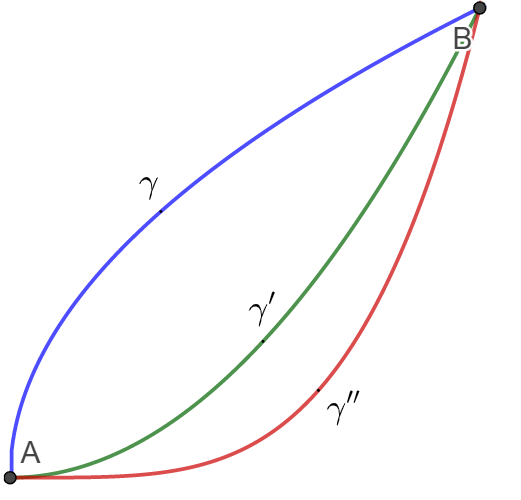
\includegraphics[width=.78\linewidth]{../figures/lec-24.1.png}
    \caption{Paths from A to B}
\end{wrapfigure}

Evaluating the LHS gives,
\begin{align*}
    \int_c \vec{\nabla}f\cdot d\vec{r} & \overset{\mathrm{(1)}}{=} \int_a^b \nabla f(r(t)) \cdot r'(t) dt      \\
                                       & = \int_a^b \left(\sum_{i=1}^{n} \pdv{f}{r_i}\times r_i'(t) \right) dt \\
                                       & =\int_a^b \dv{t}(f(r(t))) dt                                          \\
                                       & = f(r(b)) - f(r(a))                                                   \\
                                       & = f(B) - f(A)
\end{align*}
\begin{center}
    (1) follows from (\ref{eq:3}).
\end{center}


$\bullet$ This result has an important consequence that we often use in Physics.

``Work done by a conservative force always depends on the \textcolor{violet}{starting point} and the \textcolor{violet}{end point}, not on the path followed by the particle.''
\vspace*{0.2cm}

$\bullet$ We know if the force is conservative then we can define potential energy $U$ as $ \vec{F} = -\vec{\nabla}U$. Work done by the force is simply the change of potential.

\vspace*{0.2cm}

Now we will recall the basics of the ``Planes and Normals''.

\vspace*{0.2cm}

\section{Planes and Normals}
Let, $\vec{P_0} = \langle x_0,y_0,z_0 \rangle$ be a fixed vector in $\R^3$. $\vec{N} = \langle a,b,c \rangle \neq \vec{0}$. The plane through $\vec{P_0}$ with $\vec{N}$ as normal to this plane is,
$$ := \{\vec{P_0} + \vec{P} | \vec{P}\cdot \vec{N} = 0\} = \{\vec{r} | (\vec{r}-\vec{P_0})\cdot \vec{N} = 0 \} $$

\underline{\textbf{Equation of the plane}:} Consider an arbitrary point $\vec{P} = \langle x,y,z\rangle$ on the plane then, $$\langle x-x_0,y-y_0,z-z_0\rangle \cdot \langle a,b,c \rangle = 0$$

So, equation of the plane is
\begin{equation}
    a(x-x_0)+b(y-y_0) +c(z-z_0)= 0 \label{eq:4}
\end{equation}

\vspace{1cm}

Let $\vec{Q_1},\vec{Q_2}$ be independent in $\R^3$ and also satisfying $\vec{Q_i} \cdot \vec{N} = 0$. Clearly, $\vec{Q_1}\times \vec{Q_2} \neq \vec{0}$. We can see $(\vec{Q_1}\times \vec{Q_2}) \cdot \vec{Q_i} = 0$, i.e., $\{\vec{Q_1},\vec{Q_2},\vec{Q_1}\times \vec{Q_2}\}$ form a basis of $\R^3$.

$$\therefore \hspace{0.2cm}\vec{Q_1}\times \vec{Q_2} = c \vec{N}$$
So, $\{\vec{P_0} + r_1 \vec{Q_1} + r_2 \vec{Q_2} | r_1,r_2 \in \R \}$ describes the same plane as (\ref{eq:4}).

\section{Surface and Surface Integrals}

\begin{Def}{Region}{}
    A subset $\mathcal{R} \subseteq \R^2$ is called a \enquote{Region} if $\mathcal{R}$ is Open ans $\mathcal{R}$ has an area (i.e. $\partial \mathcal{R}$ is \textbf{content zero})
\end{Def}

\begin{Def}{Parametrized Surface}{ps}
    $\mathcal{L}$et $\mathcal{R} \subseteq \R^2$ be a region. $\mathcal{A}$ $C^1$ function $r:\mathcal{R} \to \R^3$ said to be a \enquote{Parametrized Surface} if :
    \begin{itemize}
        \item The component functions $r_i$ have bounded partials
        \item $r$ is $1-1$ function
        \item $\pdv{\vec{r}}{u} \times \pdv{\vec{r}}{v} \neq \vec{0}$ for all $(u,v) \in \R^2$. This means total derivative of $r$ has rank $2$.
    \end{itemize}
    $\$$ We will call range of $r$ as a \textbf{Surface}, $ \mathcal{S} = \ran(r)$.
\end{Def}

Let, $\eta$ be a map defined on $(-\varepsilon,\varepsilon)$ that maps $t \overset{\eta}{\mapsto} r(u_o=0 + t,v_0)$. Clearly, $\eta$ defines smooth curve on $\mathcal{S}$. Similarly, we can define $\tilde{\eta}$ on $(-\varepsilon,\varepsilon)$ that maps $t \overset{\tilde{\eta}}{\mapsto} r(u_0,v_0+t)$.

\begin{wrapfigure}{r}{0.5\textwidth}
    \centering
    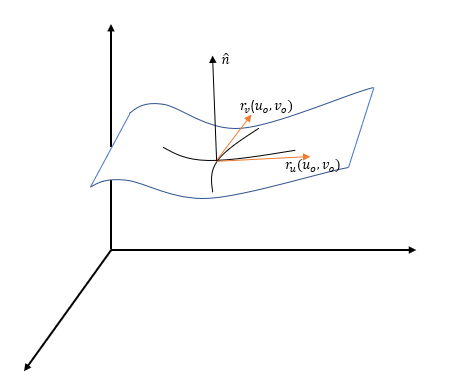
\includegraphics[width=.78\linewidth]{../figures/lec-24.2.png}
    \caption{\label{fig24:1}}
\end{wrapfigure}

Thus, $\tilde{\eta}$ also defines a smooth curve on $\mathcal{S}$.

From the figure \ref{fig24:1} we can see $\eta$ and $\tilde{\eta}$ are the curves. $r_u(u_0,v_0)=\dv{\eta}{t}\eval_{t=0}$, which gives the tangent of the curve $\eta$ at point $(u_0,v_0)$ along $x$ axis.

Similarly, for $\tilde{\eta}$, $r_v(u_0,v_0)$  gives the tangent of $\tilde{\eta}$ along $y$ axis. The vectors $r_u(u_0,v_0),r_v(u_0,v_0)$ spanned together to form a plane. This plane is known as \textbf{Tangent Plane}.

Since $r$ is $C^1$, both $\vec{r_u}$ and $\vec{r_v}$ are continuous and hence $\vec{r_u} \times \vec{r_v}$ is continuous. Also, $\vec{r_u} \times \vec{r_v}$ is along the normal vector of $\mathcal{S}$ at $r(u_0,v_0)$.

$\#$ The above statement follows from the previous section.

Now we will move towards a very important definition.

\begin{Def}{Tangent Plane}{}
    For a Parametrized Surface $r$, let $\ran(r)=\mathcal{S}$ and $r(u_0,v_0)=P$, then the plane generated by $r_u(u_0,v_0)$ and $r_v(u_0,v_0)$ through $r(u_0,v_0)$ is called the \textbf{Tangent Plane} of $\mathcal{S}$ through $P$.

    $\$$ We denote it by $T_P\mathcal{S}$.

    $\$$ Every element of $T_P\mathcal{S}$ is called \textbf{Tangent Vectors} at $P$ on $\mathcal{S}$.
\end{Def}

$\bullet$ It can be shown that $T_P\mathcal{S}$ is independent of $\mathcal{S}$'s parametrization. i.e. $T_P\mathcal{S}$ is independent of $r$ (\textbf{Homework}). Actually, for different $\tilde{r}$ of $\mathcal{S}$ the basis for $T_P\mathcal{S}$ will be changed. But they will still generate the same plane.

\vspace{0.2cm}

We will go through some examples.

\begin{Eg}{Graph of Function}{groffn}
    Let $f : \mathcal{O}_2 \to \R$ be a $C^1$ function then the graph of $f$ is $\mathcal{G}(f) = \{ (x,y,f(x,y)) : (x,y)\in \mathcal{O}_2\}$. Under the conditions $\mathcal{O}_2$ is bounded and partial derivatives of $f$ is bounded, we want to find a parametrization of this Surface $\mathcal{G}(f)$.

    \textit{Answer.} Here, we use the trivial parametrization $r : \mathcal{O}_2 \to \R^3$ that is $ r(x,y) = (x,y,f(x,y))$. Clearly, $r$ is one - one. Now, $r_u(u,v) = (1,0,f_u)$ and $r_v(u,v) = (0,1,f_v)$.

    So, $ r_u \times r_v = (-f_u,-f_v,1) \neq \vec{0}$. So, it is a parametrization of the surface.
\end{Eg}

\begin{Eg}{Torus}{}
    \begin{figure}[H]
        \centering
        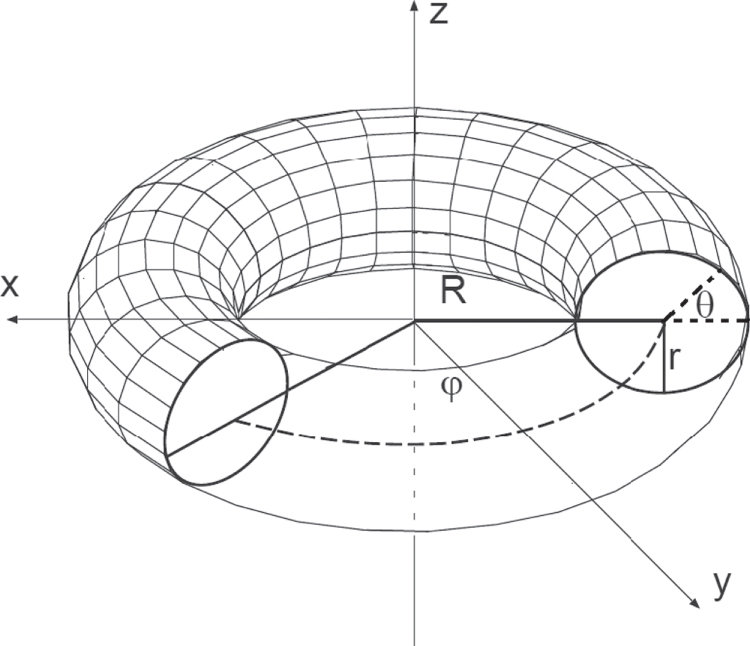
\includegraphics[width=0.5\textwidth]{../figures/lec-24.3.png}
        \caption{Torus.}
    \end{figure}

    Parametrization is given by, ($0<r<R$)
    \begin{align} \label{eq:5}
        r(\theta, \varphi) & = ((R+r\cos \theta)\cos \varphi,(R+r\cos \theta)\sin \varphi, r \sin \theta) ; 0\le \theta, \varphi \le 2\pi
    \end{align}
\end{Eg}

\begin{Eg}{Surface of Revolution}{}
    Let,$f,g$ be $C^1$ functions on $[0,b]$. Consider the curve $t \mapsto (0,f(t),g(t))$ is a $C^1$ curve. If we rotate the curve with respect to $z$ axis, we must get a surface. Parametrization  of the surface is given by,
    \[r(u,v) = (f(u)\cos v,f(u)\sin v,g(u)) \hspace{0.2cm}; u \in [0,b], v \in [0,2\pi] \]
\end{Eg}

\hspace*{0.5cm} \textbf{Exercise.} Find the Parametrization of a sphere of radius $R$.
\end{document}